%--------------------
% Packages
% -------------------
\documentclass[12pt,letterpaper]{article}
\title{Dynamic Strings, Dynamic Solutions: 
    \\\Large Applying Dynamic Programming Principles\\to String Transformation and Correction}
\author{Emma Lee}
\date{February 2024}

\usepackage[
backend=biber,
style=apa,
]{biblatex}
\addbibresource{references.bib} %Imports bibliography file

\usepackage[pdftex]{graphicx} % Required for including pictures
\graphicspath{ {./images/} }

%\usepackage[utf8x]{inputenc}
\usepackage{textcomp}
\usepackage[T1]{fontenc}
%\usepackage{gentium}
\usepackage{mathptmx} % Use Times Font
\usepackage{spverbatim}

\usepackage[bottom]{footmisc}
\usepackage[pdftex,linkcolor=black,pdfborder={0 0 0}]{hyperref} % Format links for pdf
\usepackage{calc} % To reset the counter in the document after title page
\usepackage{enumitem} % Includes lists

\frenchspacing % No double spacing between sentences
\linespread{1} % Set linespace
\usepackage[letterpaper, margin=1.5in]{geometry} %margins
%\usepackage{parskip}

\usepackage[all]{nowidow} % Tries to remove widows
\usepackage[protrusion=true,expansion=true]{microtype} % Improves typography, load after fontpackage is selected

\usepackage{lipsum} % Used for inserting dummy 'Lorem ipsum' text into the template




%-----------------------
% Set pdf information and add title, fill in the fields
%-----------------------
\hypersetup{ 	
pdfsubject = {},
pdftitle = {},
pdfauthor = {}
}

%-----------------------
% Begin document
%-----------------------
\begin{document}
\maketitle

\section{Introduction}
In any search for “the best”— the best route to take to get to work, the best TV series to watch, the best ice cream flavor, etc.— one must go through the painstaking process of trial and error. I’m a picky ice cream eater, so every time I buy ice cream, I have to try 75\% of the flavors to successfully pick one that I enjoy. Trying a bunch of different flavors over and over again can be costly (especially if the shop does not give out free samples), but if I could just remember what flavors I liked or didn’t like, I could save so much time, money, and effort. 

In the less tasty world of programming, dynamic programming enables us to save costs by doing exactly what I fail to do: remember. For large problems that are repetitive by nature, dynamic programming offers more efficiency when finding a solution. Dynamic programming takes a large problem, breaks it down into subproblems, finds the best solutions to the subproblems, remembers said solutions, and reuses those solutions to avoid unnecessary and costly, redundant computations. In other words, dynamic programming gives us optimal solutions faster, and its scope goes way beyond ice cream sampling. (Think DNA sequencing, travel route optimization, language prediction, and more!)

Ultimately, this report will explore how dynamic programming operates quickly and optimally by applying it to string transformation algorithms that help match a typo with its least costly/most likely correction.

\section{Introduction to Dynamic Programming}
To better understand dynamic programming, let’s pick apart a more concrete example: finding the nth number in the Fibonacci sequence. (based on an example from \cite{sugishita})

\begin{small}
    \begin{spverbatim}
    The Fibonacci sequence looks something like:
        1, 1, 2, 3, 5, 8, 13, …
    Where F1 and F2 = 1 and Fn = Fn-2 + Fn-1 (the next number in the 
    sequence is equal to the sum of the two numbers before it)
    \end{spverbatim}
\end{small}

A naive recursive algorithm for finding the nth Fibonacci number that does not employ dynamic programming could look something like so:

\begin{small}
    \begin{spverbatim}
    Given a positive integer n, call method fib(n) to   
    return the nth Fibonacci number where fib(n) looks like

    1	If n ==  1 or n == 2, let result = 1
    2	Otherwise, let result = fib(n-1) + fib(n-2)
    3	Return result
    \end{spverbatim}
\end{small}

\begin{footnotesize}
    \textbf{Figure 1:} Naive recursive algorithm for finding the nth Fibonacci number
\end{footnotesize}
\paragraph{}

This algorithm works, but it wastes a lot of time repeating work during the two recursive calls on line 2. For example, if we wanted to find the 5th Fibonacci number, calling fib(5) would result in the other calls to our function `fib` shown in Figure 2:

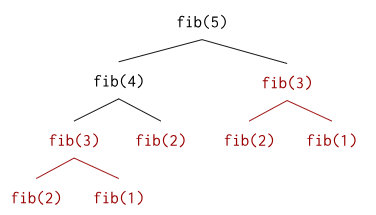
\includegraphics[scale=0.65]{images/fig2fib.png}
\paragraph{}
\begin{footnotesize}
    \noindent\textbf{Figure 2:} Diagram of the recursive calls triggered by calling `fib(5)` using the algorithm described in Figure 1. Calls colored in red indicate unnecessary, repeated work.
\end{footnotesize}
\paragraph{}

Figure 2 highlights in red how the work to compute some of the recursive calls will be duplicated if we use this naive algorithm. For example, the work to find the result of `fib(3)` has to be done twice. This approach takes valuable runtime and wastes it on doing work that has already or will already be done. This only gets worse when we give this algorithm a bigger problem, say fib(1,000,000).

A simple solution to prevent duplicate work is to remember the intermediate results. In the Figure 3 example, if we store the results of one branch’s `fib(3)`, we can save time by reusing that result when it comes up again.

This is where dynamic programming comes into play. An algorithm to solve the nth Fibonacci number problem which utilizes dynamic programming may look as follows:

\begin{small}
    \begin{spverbatim}
    Given a positive integer n (representing the 
    nth Fibonacci number to be calculated)

        Initialize an array A of size n that will store intermediate results 
        of calls to the `fib` method.
        Define a method fib(n, A) that takes in the positive integer n 
        and the initialized array where
            fib(n, A):
                If A[n] != null return A[n] 
                // reuse the previously computed solution if available
                If n == 1 or n == 2 let result = 1
                Otherwise, let result = fib(n-1) + fib(n-2)
                A[n] = result // store the computed result for future use
                Return result
    \end{spverbatim}
\end{small}

\begin{footnotesize}
    \textbf{Figure 3:} Algorithm to find the nth Fibonacci number using dynamic programming principles.
\end{footnotesize}
\paragraph{}

The algorithm described in Figure 3 makes use of the array A to store Fibonacci numbers computed along the way for later reuse so that, unlike the algorithm described in Figure 1, duplicate computations are no longer required.

\paragraph{}
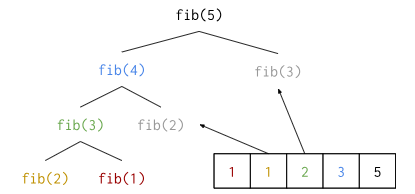
\includegraphics[scale=0.65]{images/fig4fib2.png}
\paragraph{}
\begin{footnotesize}
    \noindent\textbf{Figure 4:} Diagram of the recursive calls triggered by calling `fib(5)` using the algorithm described in Figure 3. Note how repeated recursive calls draw from stored memory instead of recomputing previously computed solutions.
\end{footnotesize}
\paragraph{}

As seen in Figure 4, when applying the dynamic programming algorithm, instead of needing to recompute results, we can instead just draw from the previously computed and stored results. Thus, we spend less time doing unnecessary computations and can get to our solution faster.

Dynamic programming not only leads to faster solutions– it also leads to optimal ones.

Many problems concerned with optimization exhibit optimal substructure property. (i.e. finding the shortest path to get from location A to location B while hitting various stops in between, scheduling daily tasks to maximize productivity, selecting what items to pack so that you could fit the most in your suitcase, etc.) GeeksforGeeks explains that a “given problem is said to have Optimal Substructure Property if the optimal solution of the given problem can be obtained by using the optimal solution to its subproblems instead of trying every possible way to solve the subproblems” (\cite{geeksforgeeks}). The idea is that if you find the optimal solutions to smaller instances of a problem and add them all up, you will end up with the optimal solution to the whole, larger problem.

Because dynamic programming involves the breaking down of a larger problem into subproblems (and solving each subproblem once), if a dynamic programming algorithm focuses on computing the optimal solution for a given subproblem, by the end, the algorithm will result in the optimal solution for the entire problem.

\section{Introduction to Cormen’s String Transformation Algorithms}
To better understand how dynamic programming results in optimal solutions, consider Cormen’s following algorithms to find the least costly way to transform a string $x$ into another string $y$.

The algorithm Cormen describes in Figure 5 (below) uses dynamic programming by breaking down the given strings $x$ and $y$ into subproblems focused in on prefixes. The idea is that in order to find the optimal/least costly way to transform string $x$ into string $y$, we can just find the least costly way to transform prefix $x_i$ into prefix $y_j$ (where $i$ goes from 0 to length of $x$ and $j$ from 0 to length of $y$). We break the string problem into string prefix subproblems, and for each subproblem, we find the optimal solution and store it for later use. 

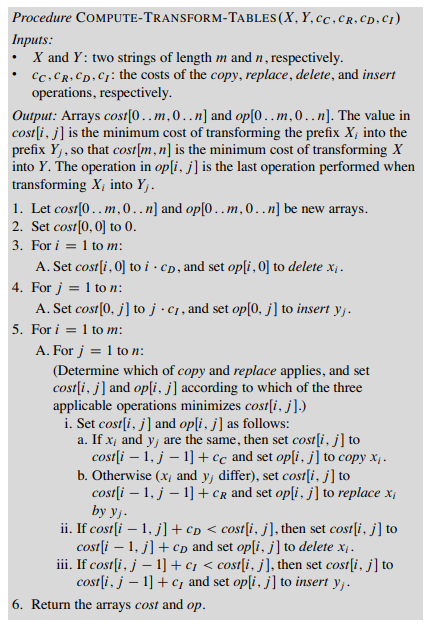
\includegraphics[scale=0.8]{images/cormenalgo1.png}
\paragraph{}
\begin{footnotesize}
    \noindent\textbf{Figure 5:} Cormen's algorithm to compute the lowest cost operations to transform one string into another. Taken from \textit{Algorithms Unlocked} (\cite{cormen}).
\end{footnotesize}
\paragraph{}

To store the optimal solutions to each prefix subproblem, the COMPUTE-TRANSFORM-TABLES algorithm generates two matrices: one to track costs and one to track operations. 

Costs refer to how “expensive” an operation may be, where an operation is one of the 4 options: \textit{copy, replace, delete, or insert}. For instance, a \textit{copy} operation would be cheaper than a \textit{replace} operation because it does not result in changes to the original string. One would perform a \textit{copy} operation if the specific character they’re looking at in one string matches in character and position when compared to the other string. A \textit{replace} operation is more expensive (takes more effort) than a \textit{copy} operation because it involves changing a character in one string, but it is less costly than \textit{delete} or \textit{insert} operations because it does not disrupt string lengths. Cormen gives these 4 operations the following costs: -1, +1, +3, and +3 (where -1 is for a \textit{copy}, +1 for a \textit{replace}, and so on)\footnote[1]{More on Cormen’s cost assignments can be found in his book (Algorithms Unlocked, 122-123).}. Keep in mind that when we put the 4 operation options in the context of a specific prefix subproblem, a generally more costly operation (like \textit{replace}) may actually be better/cheaper choice in the grander scheme of things. Generally cheaper operations like \textit{copy} may not always be applicable. Additionally, performing certain operations on one prefix subproblem may open up other possible operations on future subproblems. In other words, optimal solutions to one subproblem may be dependent on the result of another.

So, when Figure 5’s algorithm computes the cheapest cost and cheapest operation for given prefixes, the algorithm often has to look back at the costs of previous prefix transformations. This is where the matrices come into play. The algorithm in Figure 5 fills the cost matrix so that `cost[i][j]` contains the cheapest cost of transforming prefix $x_i$ into prefix $y_j$. The operations matrix is likewise filled so that `op[i][j]` contains the cheapest operation used to transform prefix $x_i$ into prefix $y_j$. By storing these intermediate results in the cost and operations matrices, Cormen’s algorithm avoids recalculating the same subproblems and is thus a prime example of the power of dynamic programming.

By the end of the algorithm, the right-most and bottom-most element in the cost matrix will contain the lowest cost of transforming the entire string $x$ into $y$, giving us the answer to the lowest string transformation cost problem. However, in order to find the actual least costly sequence of operations to perform on the strings, we need to use Cormen’s second algorithm shown in Figure 6.

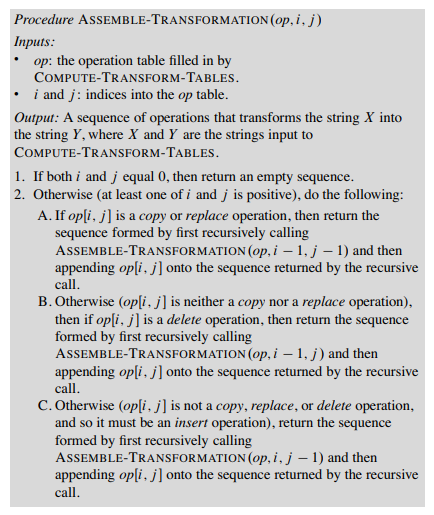
\includegraphics[scale=0.8]{images/cormenalgo2.png}
\paragraph{}
\begin{footnotesize}
    \noindent\textbf{Figure 6:} Cormen's algorithm to reconstruct the lowest cost operations sequence to transform one string into another. Taken from \textit{Algorithms Unlocked} (\cite{cormen}).
\end{footnotesize}
\paragraph{}

Figure 6’s algorithm is purely a reconstructive one; it does not know for sure that the operations in the operation matrix provided by Figure 5 are the least costly ones. (That is the job of Figure 5’s algorithm.) Rather, Figure 6 is concerned with using the information in the operation matrix to string together the least costly sequence of operations needed to transform string $x$ into string $y$. It starts at the end (bottom-most and right-most corner) and recursively backtracks through the matrix. Figure 6’s algorithm looks at the last operation in the operation matrix, and, from there, it determines how to adjust its indexing to find the next operation. For more clarity on how this algorithm works, we will walk through an example later in this report.

In short, the ASSEMBLE-TRANSFORMATION algorithm recurses through the given operations table to output the sequence of operations to transform string $x$ into $y$. Because it uses COMPUTE-TRANSFORM-TABLES output, the operation sequence it outputs ends up being the least costly transformation sequence.
\paragraph{}
We will put these two algorithms to the test, applying their optimal string transformation sequence output to a typo correction/predicting program.


\section{Typo Correction Program - Methodology}
The program described in Figure 7 takes user input words (which we assume may contain typos) and searches a file of words\footnote[2]{File of words can be found in /home/gtowell/Public/CS337/Lab03/words.} to produce the “most likely” spelling corrections. A “most likely” correction for a given word $x$ is a word $y$ such that $y$ is a string with the lowest cost transformation from $x$. The cost to transform $x$ into $y$ should be the lowest when compared to the cost to transform $x$ into any other string in the file (disregarding strings with duplicate transformation costs). I’ve implemented the program in Go using an algorithm that looks like the following:

\begin{small}
    \begin{spverbatim}
    Parse the file of words and store in an array of strings
    For each (potentially misspelled) word taken from the command line
    \end{spverbatim}
    \begin{enumerate}[nosep]
        \item \begin{spverbatim}set the initial lowestCostWord to be the first word in the array\end{spverbatim}
        \item \begin{spverbatim}calculate the lowest cost of transforming the potentially mispelled word to the initial lowestCostWord by using Cormen’s COMPUTE-TRANSFORM-TABLES algorithm\end{spverbatim}
        \item \begin{spverbatim}set this calculated cost to the initial lowestCost\end{spverbatim}
        \item \begin{spverbatim}[optional, for debug] use Cormen’s ASSEMBLE-TRANSFORMATION algorithm to reconstruct the least costly transformation sequence\end{spverbatim}
        \item \begin{spverbatim}For each subsequent word in words\end{spverbatim}
            \begin{enumerate}
                \item \begin{spverbatim}calculate the lowest cost of transforming the potentially mispelled word to this subsequent word usimg Cormen’s COMPUTE-TRANSFORM-TABLES algorithm\end{spverbatim}
                \item \begin{spverbatim}[optional, for debug] use Cormen’s ASSEMBLE-TRANSFORMATION algorithm to reconstruct the least costly transformation sequence\end{spverbatim}
                \item \begin{spverbatim}if the computed cost is < the initial lowestCost\end{spverbatim}
                    \begin{spverbatim}set lowestCost = the computed cost\end{spverbatim}
                    \begin{spverbatim}set lowestCostWord = this subsequent word\end{spverbatim}
            \end{enumerate}
        \item \begin{spverbatim}Print the lowestCostWord and its corresponding lowestCost\end{spverbatim}
    \end{enumerate}
\end{small}

\paragraph{}
\begin{footnotesize}
    \textbf{Figure 7:} Description of a program to search a file of words to find a "most likely" match for a user given typo. A "most likely" word refers to a word with the lowest cost of transformation and can be thought as a word that is closest to/most similar to the user given typo.
\end{footnotesize}
\paragraph{}

Since the program described in Figure 7 is intended to search a words file to find the most likely spelling correction for a given typo, Cormen’s predefined costs for operations (-1, +1, +3, +3) are no longer ideal. Under the premise that typos occur when a user accidentally hits a key close to the intended key instead of the intended key itself, we’d expect that replace operation costs are no longer constant. For instance, mistyping the letter ‘a’ by accidentally pressing letter key ‘s’ (which is one key off on a standard US keyboard), is much more likely than mistyping ‘a’ by pressing ‘p’ (which is across the standard US keyboard). Calculating replacement cost based on keyboard distance and other contributing factors would be ideal, but that’s a topic for future work. For now, the program described in Figure 7 will compute replacement cost using an arbitrary formula to simulate replacement cost discrepancy.

\begin{small}
    \begin{spverbatim}
    The formula looks like:
    		sqrt(abs(iA - iB)) + 1
    where iA is the integer representation/ASCII value of a given
    character A and where iB is similarly the integer representation 
    of given character B
    \end{spverbatim}
\end{small}
    
Thus, when applying Cormen’s COMPUTE-TRANSFORM-TABLES algorithm, the values for each operation will be as follows:

\begin{small}
    \begin{spverbatim}
    cost of copy: 0
    cost of replace: -99 
        // a placeholder for the computed value using the formula above
    cost of delete: 3
    cost of insert: 3
    \end{spverbatim}
\end{small}

The reasons for choosing these specific values (namely 0 and 3) are relatively arbitrary. However, the weighing of these values (in the sense that copy costs less than delete and insert and should cost less than replace according to the replacement cost formula) maintains the logical idea that operations that alter the strings less are cheaper.

I translated Cormen’s algorithms to Go code, and used those implementations alongside the program described in Figure 7, testing it with various command line inputs\footnote[3]{Other runs with additional command line inputs can be found in Appendices A, B, and C.}. We will be focusing on the command line input: `Needier moare ars onw comend liine`

\section{Analysis of Output Given Command Line Input: `Needier moare ars onw comend liine`}
When given the following command line input:  `Needier moare ars onw comend liine`, the program produces the following output:

\begin{small}
    \begin{spverbatim}
    Needier -> Seeder with cost 6
    moare -> mare with cost 3
    ars -> art with cost 2
    onw -> on with cost 3
    comend -> commend with cost 3
    liine -> ligne with cost 2
    \end{spverbatim}
\end{small}

\begin{footnotesize}
    \textbf{Figure 8:} Output from running the program described in Figure 7 with the following command line input: `Needier moare ars onw comend liine`.
\end{footnotesize}
\paragraph{}

According to Figure 8, the most likely spelling correction for “ars” which can be found in the words file is “art.” To see why, let’s pick apart Cormen’s COMPUTE-TRANSFORM-TABLES algorithm.

\subsection{Cormen’s COMPUTE-TRANSFORM-TABLES Algorithm with an Example}
Let’s look at the cost and operation matrices for transforming “ars” into “art” (resulting from code found in Appendix E):

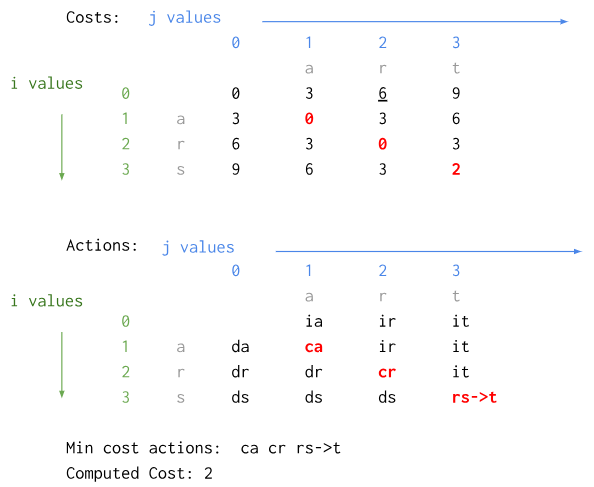
\includegraphics[scale=0.7]{images/fig9example1.png}
\paragraph{}
\begin{footnotesize}
    \noindent\textbf{Figure 9:} The cost and operations matrices generated by running Cormen's COMPUTE-TRANSFORM-TABLES algorithm on strings "ars" and "art". $i$ values iterate through the string "ars" while $j$ values iterate through "art". In the actions table, the 4 operations (copy, replace, delete, insert) are abbreviated using the first letter of the operation followed by the letter(s) involved during the operation. Values highlighted in red indicate lowest cost subproblem solutions.
\end{footnotesize}
\paragraph{}

Figure 9 shows the cost and operations matrices generated by Cormen’s algorithm as described in Figure 5. String $x$ refers to the string “args” and string $y$ refers to the string “art.” Recall that every element in the cost matrix is indexed at `cost[i][j]` such that for a string prefix of $x$ (from character 0 to character $i$), the cheapest cost to transform said prefix into a prefix of $y$ (from 0 to $j$) is stored. The operations matrix is likewise indexed but handles the least costly operations rather than the actual minimum cost. 

In Figure 9, consider each $i$ value as a position in a string $x$, “ars,”  and each $j$ value as a position in a string $y$, “art.” When $i$ is 0, only insert operations are being performed. This is because, when $i$ is 0, the algorithm looks at a prefix $ars_0$ (or the prefix of the string “ars” from 0 to 0, which is empty “”). Thus, to transform $ars_0$ to prefix $art_1$, $art_2$, and so on, we must insert characters from $art$. On the other hand, when $j$ is 0, the algorithm is looking for ways to convert prefixes $ars_1$, $ars_2$, and so on into prefix $art_0$ (also an empty string). To do this, we have to delete characters from ars.

Moreover, if we look at the cost elements when $i$ or $j$ are 0, we can observe each value getting incremented by 3. This is because the algorithm considers previously computed costs for previous prefixes when finding the optimal solution for a given prefix. (Recall that this string transformation problem exhibits optimal substructure property in which the optimal solution to a large problem can be found from a combination of the optimal solutions to smaller subproblems.) So, for position [0][2] (underlined in Figure 9), for example, the computed minimum cost to transform $ars_0$ (an empty string “”) to $art_2$ (“ar”) is 6. This value 6 is based on the minimum cost to transform “” to “a” plus the minimum cost to transform “” to “r”. Both of these are insert operations and thus have a cost of 3 (3+3 = 6). A similar logic applies to the rest of the matrix.

If we look at the cost matrix in Figure 9, when $i$ is 1 and $j$ is 1, we’re dealing with the prefix of $ars_1$ (which is the character ‘a’) and the prefix of $art_1$ (which is also the character ’a’). Since these characters are the same, only a copy operation must be performed to transform the prefix $ars_1$ into $art_1$. Hence, stored in the matrices at index [1][1] is the cost of copying (0) and the copy operation, followed by the character being copied (ca). Knowing that copying is generally the cheapest operation, at index [1][1] we have found and stored the least costly operation and the minimum cost of transforming $ars_1$ into $art_1$. 

Later on, when the algorithm encounters the subproblem dealing with prefixes $ars_2$ (“ar”) and $art_2$ (“ar”), it knows that to find the optimal solution/cheapest transformation, it should compute the cheapest way to transform ‘r’ into ‘r’ (which is another copy operation with cost 0) and add that value to the cheapest way to transform the previous prefix transformation (copy ‘a’ with cost 0).

This process happens repeatedly until the algorithm reaches the end of both strings. The cost stored at position [3][3] in the matrix is thus the minimum cost to convert $ars$ into $art$.

\subsection{Cormen’s ASSEMBLE-TRANSFORMATION Algorithm with an Example}
Now that we’ve walked through Cormen’s first transformation algorithm with an example, let’s look at another to better understand how Cormen’s second algorithm reconstructs the cheapest transformation sequence.

Consider transforming the typo “Needier” into the most likely correction “Seeder”:

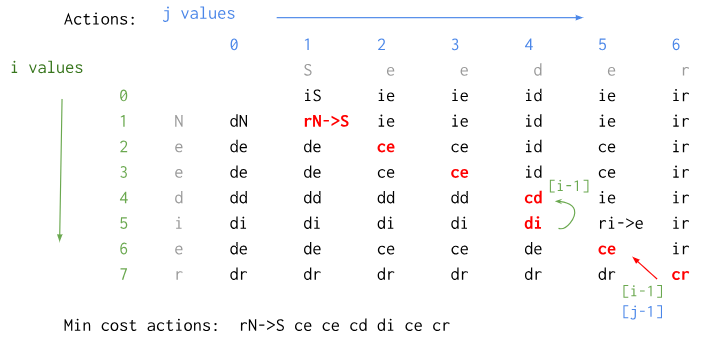
\includegraphics[scale=0.7]{images/fig10example2.png}
\paragraph{}
\begin{footnotesize}
    \noindent\textbf{Figure 10:} The operations matrix generated by running Cormen's COMPUTE-TRANSFORM-TABLES algorithm on strings "Needier" and "Seeder".
\end{footnotesize}
\paragraph{}

For the operations matrix generated in Figure 10, Cormen’s ASSEMBLE-TRANSFORMATION algorithm starts at position [7][6] and handles the prefixes $Needier_7$ (which is “Needier”) and $Seeder_6$ (which is “Seeder”). It sees that the operation stored at that position is $cr$, a \textit{copy} operation to copy the letter ‘r’ from $Needier$ to the $Seeder$ string.

Because the algorithm encountered a \textit{copy} operation, it knows that the character at position 7 in $Needier$ is the same as the one found at position 6 in $Seeder$, so it recognizes that the string lengths/positioning were not altered. Thus, the algorithm can simply move backward and recur on position [7-1][6-1], or [i-1][j-1]. The same goes for \textit{replace} operations.

The algorithm does this and sees that the operation at position [6][5] is also a \textit{copy}, so it similarly recurs on [i-1][j-1], or [5][4]. However, here, it sees a \textit{delete} operation, and it recognizes that the ‘i’ from $Needier$ (at position 5) is deleted, so the string length of $Needier$ has been shortened. To account for this length shortening/position change, the algorithm recurs on [i-1] but maintains its position in $Seeder$ at position [j]. A similar procedure is applied for insert operations.

Cormen’s algorithm continues calling itself recursively on adjusted indices to traverse the operation matrix until it reaches position [0][0]. From there, it will append all the operations to a string for return.

\section{Summary}
By now, we’ve explored the concept of dynamic programming and how it breaks down large problems into smaller ones while storing intermediate solutions to avoid repetitive computations. We also discussed two of Cormen’s string transformation algorithms that employ dynamic programming and have also applied these algorithms to a program that finds the most likely correction to a user-inputted typo. Lastly, we’ve walked through two typo examples to better understand how Cormen’s algorithms compute the lowest cost and reconstruct the lowest cost transformation sequence.

\section{Future Work}
Regarding the typo-correction problem, the arbitrary replacement cost formula (described in the methodology section) should ideally be enhanced to improve accuracy and/or real-life utility. Factors like the distance between characters on a keyboard, common misspellings, case sensitivity, or the level of phonetic similarity between two characters should be taken into consideration when determining replacement costs.

%Where the bibliography will be printed
  \printbibliography

\pagebreak
\section*{Appendices}
\subsection*{Appendix A}
    Output generated when running the typo correction program on the given command line input: `thefact factotum`.
    \begin{footnotesize}
        \begin{verbatim}
        thefact -> theat with cost 6
        factotum -> factotum with cost 0
        \end{verbatim}
    \end{footnotesize}
    
\subsection*{Appendix B}
    Output generated when running the typo correction program on the given command line input: `thesis theorem`.
    \begin{footnotesize}
        \begin{verbatim}
        thesis -> thesis with cost 0
        theorem -> theorem with cost 0
        \end{verbatim}
    \end{footnotesize}
    
\subsection*{Appendix C}
    Output generated when running the typo correction program on the given command line input: `repurt derrrbing teh algorms usig fololwing inupts`.
    \begin{footnotesize}
        \begin{verbatim}
        repurt -> report with cost 3
        derrrbing -> absorbing with cost 8
        teh -> reh with cost 2
        algorms -> algosis with cost 5
        usig -> sig with cost 3
        fololwing -> following with cost 4
        inupts -> input with cost 7
        \end{verbatim}
    \end{footnotesize}
    
\pagebreak
\subsection*{Appendix D}
    (Task 1) Source code to implement Cormen's two string transformation algorithms and test using two user-inputted strings on the command line
    \begin{scriptsize}
        \begin{verbatim}
package main

import (
    "fmt"
    "os"
    "strings"
)

func computeTransformTable(x string, y string, cCost int, rCost int, dCost int, iCost int) ([][]int, [][]string) {
    m := len(x)+1
    n := len(y)+1
    cost := make([][]int, m)
    for row := range cost {
        cost[row] = make([]int, n)
    }

    op := make([][]string, m)
    for row := range op {
        op[row] = make([]string, n)
    }

    cost[0][0] = 0;

    for i := 1; i < m; i++ {
        cost[i][0] = i * dCost
        op[i][0] = "d" + string(([]rune(x))[i-1]) 
    }

    for j := 1; j < n; j++ {
        cost[0][j] = j * iCost
        op[0][j] = "i" + string(([]rune(y))[j-1]) 
    }

    for i := 1; i < m; i++ {
        for j := 1; j < n; j++ {
            if x[i-1] == y[j-1] /*&& x[i] != " "*/ { // if should copy
                cost[i][j] = cost[i-1][j-1] + cCost
                op[i][j] = "c" + string(([]rune(x))[i-1])
            } else {
                cost[i][j] = cost[i-1][j-1] + rCost
                op[i][j] = "r" + string(([]rune(x))[i-1]) + "->" + string(([]rune(y))[j-1])
            }

            if cost[i-1][j] + dCost < cost[i][j] {
                cost[i][j] = cost[i-1][j] + dCost
                op[i][j] = "d" + string(([]rune(x))[i-1])
            }

            if cost[i][j-1] + iCost < cost[i][j] {
                cost[i][j] = cost[i][j-1] + iCost
                op[i][j] = "i" + string(([]rune(y))[j-1])
            }
        }
    }

    return cost, op
}

/* given the operation table from the compute transform table output
 * performed on strings s1 and s2 and the ending indices of the op table,
 * return a sequence of needed operations to transform s1 to s2
 */
func assembleTransformation(op [][]string, i int, j int) string {
    if i == 0 && j == 0 {
        return ""
    }

    if ([]rune(op[i][j]))[0] == 'c' || ([]rune(op[i][j]))[0] == 'r' {
        return assembleTransformation(op, i-1, j-1) + " " + op[i][j] // ?????
    } else if ([]rune(op[i][j]))[0] == 'd' {
        return assembleTransformation(op, i-1, j) + " " + op[i][j]
    } else {
        return assembleTransformation(op, i, j-1) + " " + op[i][j]
    }
}

/* given a sequence of operations to transform one string to another
 * calculate the cost where copy = -1, replace = +1, delete/insert = +2
 * use to compare w/ computed lowest cost from last element in computed cost table
 */
func debugComputeCost(opSequence string) int {
    cost := 0
    seqList := strings.Split(strings.TrimSpace(opSequence), " ")
    for _, seq := range seqList {
        runes := []rune(seq)
        if runes[0] == 'c' {
            cost += -1
        } else if runes[0] == 'r' {
            cost += 1
        } else {
            cost += 2
        }
    }
    return cost
}

func main() {
    s1 := os.Args[1]
    s2 := os.Args[2]
    m := len(s1)+1
    n := len(s2)+1
	
    cost, op := computeTransformTable(s1, s2, -1, 1, 2, 2)
    result := assembleTransformation(op, m-1, n-1)

    fmt.Printf("Costs:\n")
    for row := 0; row < m; row++ {
        for column := 0; column < n; column++{
            fmt.Print(cost[row][column], "\t")
        }
        fmt.Print("\n")
    } 

    fmt.Printf("Actions:\n")
    for row := 0; row < m; row++ {
        for column := 0; column < n; column++{
            fmt.Print(op[row][column], "\t")
        }
        fmt.Print("\n")
    } 

    fmt.Printf("Min cost actions: %s\n", result)
    fmt.Printf("Computed Cost: %d\n", cost[len(s1)][len(s2)])
    fmt.Printf("Debug Computed Cost: %d\n", debugComputeCost(result))
}
        \end{verbatim}
    \end{scriptsize}

\pagebreak
\subsection*{Appendix E}
    (Task 2) Source code that builds on code found in Appendix D to account for non constant replacement costs.
    \begin{scriptsize}
        \begin{verbatim}
package main

import (
    "fmt"
    "os"
    "strings"
    "math"
)

func computeTransformTable(x string, y string, cCost int, rCost int, dCost int, iCost int) ([][]int, [][]string) {
    m := len(x)+1
    n := len(y)+1
    cost := make([][]int, m)
    for row := range cost {
        cost[row] = make([]int, n)
    }
    
    op := make([][]string, m)
    for row := range op {
        op[row] = make([]string, n)
    }
    
    cost[0][0] = 0;
    
    for i := 1; i < m; i++ {
        cost[i][0] = i * dCost
        op[i][0] = "d" + string(([]rune(x))[i-1]) 
    }
    
    for j := 1; j < n; j++ {
        cost[0][j] = j * iCost
        op[0][j] = "i" + string(([]rune(y))[j-1]) 
    }
    
    for i := 1; i < m; i++ {
        for j := 1; j < n; j++ {
            if x[i-1] == y[j-1] /*&& x[i] != " "*/ { // if should copy
                cost[i][j] = cost[i-1][j-1] + cCost
                op[i][j] = "c" + string(([]rune(x))[i-1])
            } else {
                cost[i][j] = cost[i-1][j-1] + int(considerMisspellings(([]rune(x))[i-1], ([]rune(y))[j-1]))
                op[i][j] = "r" + string(([]rune(x))[i-1]) + "->" + string(([]rune(y))[j-1])
            }
    
            if cost[i-1][j] + dCost < cost[i][j] {
                cost[i][j] = cost[i-1][j] + dCost
                op[i][j] = "d" + string(([]rune(x))[i-1])
            }
    
            if cost[i][j-1] + iCost < cost[i][j] {
                cost[i][j] = cost[i][j-1] + iCost
                op[i][j] = "i" + string(([]rune(y))[j-1])
            }
        }
    }
    
    return cost, op
}

/* given the operation table from the compute transform table output
 * performed on strings s1 and s2 and the ending indices of the op table,
 * return a sequence of needed operations to transform s1 to s2
 */
func assembleTransformation(op [][]string, i int, j int) string {
    if i == 0 && j == 0 {
        return ""
    }
    
    if ([]rune(op[i][j]))[0] == 'c' || ([]rune(op[i][j]))[0] == 'r' {
        return assembleTransformation(op, i-1, j-1) + " " + op[i][j] // ?????
    } else if ([]rune(op[i][j]))[0] == 'd' {
        return assembleTransformation(op, i-1, j) + " " + op[i][j]
    } else {
        return assembleTransformation(op, i, j-1) + " " + op[i][j]
    }
}

/* given a sequence of operations to transform one string to another
 * calculate the cost where copy = 0, replace = dependent on 
 * considerMisspellings, delete/insert = +3; use to compare w/ computed
 * lowest cost from last element in computed cost table
 */
func debugComputeCost(opSequence string) int {
    cost := 0
    seqList := strings.Split(strings.TrimSpace(opSequence), " ")
    for _, seq := range seqList {
        runes := []rune(seq)
        if runes[0] == 'r' {
            // runes[2, 3] is "->"
            cost += int(considerMisspellings(runes[1], runes[4]))
        } else if runes[0] != 'c' {
            cost += 3
        }
    }
    return cost
}

// return the cost of transforming a to b considering typo probability
func considerMisspellings(a rune, b rune) float64 {
    iA := int(a)
    iB := int(b)
    return math.Sqrt(math.Abs(float64(iA)-float64(iB))) + float64(1)
}

func main() {
    s1 := os.Args[1]
    s2 := os.Args[2]
    m := len(s1)+1
    n := len(s2)+1
    
    cost, op := computeTransformTable(s1, s2, 0, -99, 3, 3)
    result := assembleTransformation(op, m-1, n-1)
    
    fmt.Printf("Costs:\n")
    for row := 0; row < m; row++ {
        for column := 0; column < n; column++{
            fmt.Print(cost[row][column], "\t")
        }
        fmt.Print("\n")
    } 
    
    fmt.Printf("Actions:\n")
    for row := 0; row < m; row++ {
        for column := 0; column < n; column++{
            fmt.Print(op[row][column], "\t")
        }
        fmt.Print("\n")
    } 
    
    fmt.Printf("Min cost actions: %s\n", result)
    fmt.Printf("Computed Cost: %d\n", cost[m-1][n-1])
    fmt.Printf("Debug Computed Cost: %d\n", debugComputeCost(result))
}
        \end{verbatim}
    \end{scriptsize}

\pagebreak
\subsection*{Appendix F}
    (Task 3) Source code to implement a typo correction program that searches a word file to find the "most likely" corrections for user given typos.
    \begin{scriptsize}
        \begin{verbatim}
package main

import (
    "fmt"
    "os"
    "bufio"
    "strings"
    "math"
)

func computeTransformTable(x string, y string, cCost int, rCost int, dCost int, iCost int) ([][]int, [][]string) {
    m := len(x)+1
    n := len(y)+1
    cost := make([][]int, m)
    for row := range cost {
        cost[row] = make([]int, n)
    }
    
    op := make([][]string, m)
    for row := range op {
        op[row] = make([]string, n)
    }
    
    cost[0][0] = 0;
    
    for i := 1; i < m; i++ {
        cost[i][0] = i * dCost
        op[i][0] = "d" + string(([]rune(x))[i-1]) 
    }
    
    for j := 1; j < n; j++ {
        cost[0][j] = j * iCost
        op[0][j] = "i" + string(([]rune(y))[j-1]) 
    }
    
    for i := 1; i < m; i++ {
        for j := 1; j < n; j++ {
            if x[i-1] == y[j-1] /*&& x[i] != " "*/ { // if should copy
                cost[i][j] = cost[i-1][j-1] + cCost
                op[i][j] = "c" + string(([]rune(x))[i-1])
            } else {
                cost[i][j] = cost[i-1][j-1] + int(considerMisspellings(([]rune(x))[i-1], ([]rune(y))[j-1]))
                op[i][j] = "r" + string(([]rune(x))[i-1]) + "->" + string(([]rune(y))[j-1])
            }
    
            if cost[i-1][j] + dCost < cost[i][j] {
                cost[i][j] = cost[i-1][j] + dCost
                op[i][j] = "d" + string(([]rune(x))[i-1])
            }
    
            if cost[i][j-1] + iCost < cost[i][j] {
                cost[i][j] = cost[i][j-1] + iCost
                op[i][j] = "i" + string(([]rune(y))[j-1])
            }
        }
    }
    
    return cost, op
}
    
/* given the operation table from the compute transform table output
 * performed on strings s1 and s2 and the ending indices of the op table,
 * return a sequence of needed operations to transform s1 to s2
 */
func assembleTransformation(op [][]string, i int, j int) string {
    if i == 0 && j == 0 {
        return ""
    }
    
    if ([]rune(op[i][j]))[0] == 'c' || ([]rune(op[i][j]))[0] == 'r' {
        return assembleTransformation(op, i-1, j-1) + " " + op[i][j] // ?????
    } else if ([]rune(op[i][j]))[0] == 'd' {
        return assembleTransformation(op, i-1, j) + " " + op[i][j]
    } else {
        return assembleTransformation(op, i, j-1) + " " + op[i][j]
    }
}
    
/* given a sequence of operations to transform one string to another
 * calculate the cost where copy = 0, replace = dependent on 
 * considerMisspellings, delete/insert = +3; use to compare w/ computed
 * lowest cost from last element in computed cost table
 */
func debugComputeCost(opSequence string) int {
    cost := 0
    seqList := strings.Split(strings.TrimSpace(opSequence), " ")
    for _, seq := range seqList {
        runes := []rune(seq)
        if runes[0] == 'r' {
            // runes[2, 3] is "->"
            cost += int(considerMisspellings(runes[1], runes[4]))
        } else if runes[0] != 'c' {
            cost += 3
        }
    }
    return cost
}
    
// return the cost of transforming a to b considering typo probability
func considerMisspellings(a rune, b rune) float64 {
    iA := int(a)
    iB := int(b)
    return math.Sqrt(math.Abs(float64(iA)-float64(iB))) + float64(1)
}
    
func main() {
    // collect args
    stringsToConvert := os.Args[1:] // remove first arg which is program name
    
    // open file & returns os.File type pointer (or an error)
    file, error := os.Open("words")
    
    // check for error
    if error != nil {
        fmt.Printf("Error while reading the file %v\n", error)
    }
    
    scanner := bufio.NewScanner(file)
    scanner.Split(bufio.ScanLines)
    
    var words []string
    
    for scanner.Scan() {
        words = append(words, strings.TrimSpace(scanner.Text()))
    }
    
    // close the file
    file.Close()
    
    /* now have list of strings to convert & possible strings to convert to
     * find lowest cost word
     */
    for _, s1 := range stringsToConvert {
        lowestCostWord := words[0] // set lowestCostWord to first word
        cost, op := computeTransformTable(s1, lowestCostWord, 0, -99, 3, 3)
        assembleTransformation(op, len(s1), len(lowestCostWord))
        lowestCost := cost[len(s1)][len(lowestCostWord)] // set lowestCost to cost for first word
        
        for i := 1; i < len(words); i++ {
            s2 := words[i]
            m := len(s1)+1
            n := len(s2)+1
            cost, op := computeTransformTable(s1, s2, 0, -99, 3, 3)
            assembleTransformation(op, m-1, n-1)
            computedCost := cost[m-1][n-1]
            if  computedCost < lowestCost {
                lowestCostWord = s2
                lowestCost = computedCost
            }
        }
    
        fmt.Printf("%s -> %s with cost %d\n", s1, lowestCostWord, lowestCost)
    }
}
        \end{verbatim}
    \end{scriptsize}
    
\end{document}
https://www.overleaf.com/project/65c4253531c9a07b010f113c